\section{Evaluation des Baseline-Algorithmus}
\label{sec:EvaluationPhash}


\begin{figure}[H]
\centering
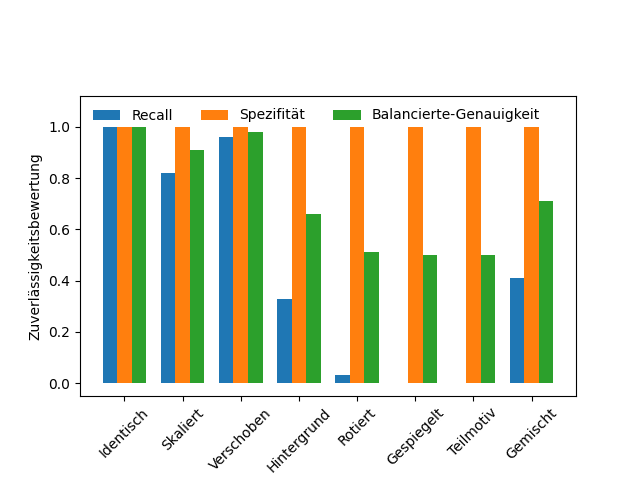
\includegraphics[scale=0.7]{Abbildungen/Evaluation/phash/standard}
\caption{Zuverl�ssigkeit des pHash Algorithmus in mehreren Szenarien}
\label{fig:phash-standard}
\end{figure}

\begin{figure}[H]
\centering
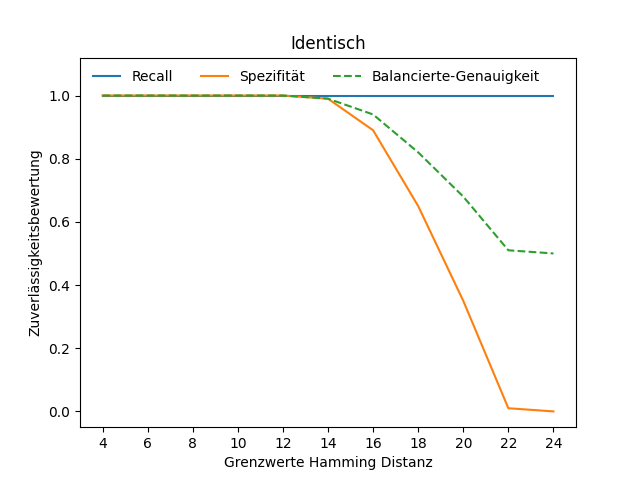
\includegraphics[scale=0.43]{Abbildungen/Evaluation/phash/identical}
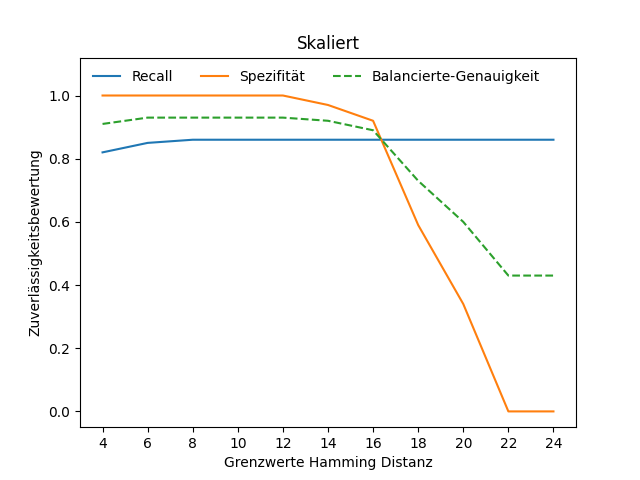
\includegraphics[scale=0.43]{Abbildungen/Evaluation/phash/scaled}
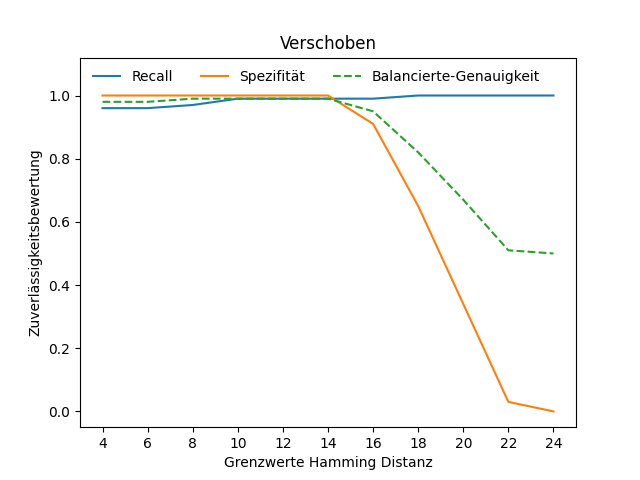
\includegraphics[scale=0.43]{Abbildungen/Evaluation/phash/moved}
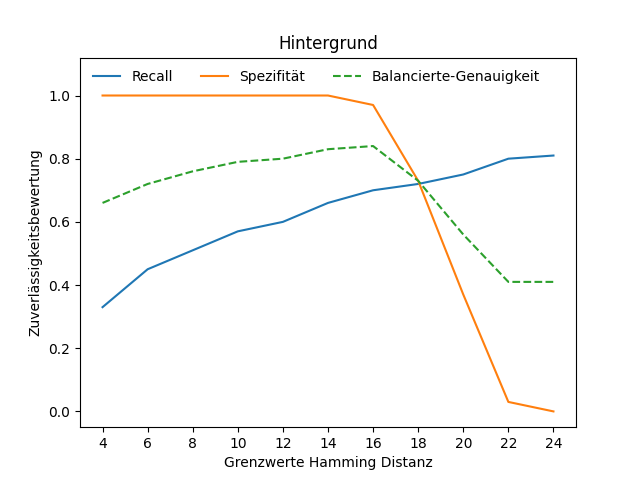
\includegraphics[scale=0.43]{Abbildungen/Evaluation/phash/background}
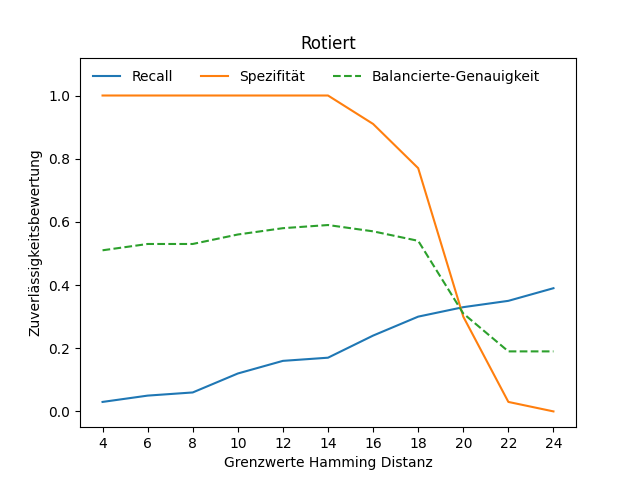
\includegraphics[scale=0.43]{Abbildungen/Evaluation/phash/rotated}
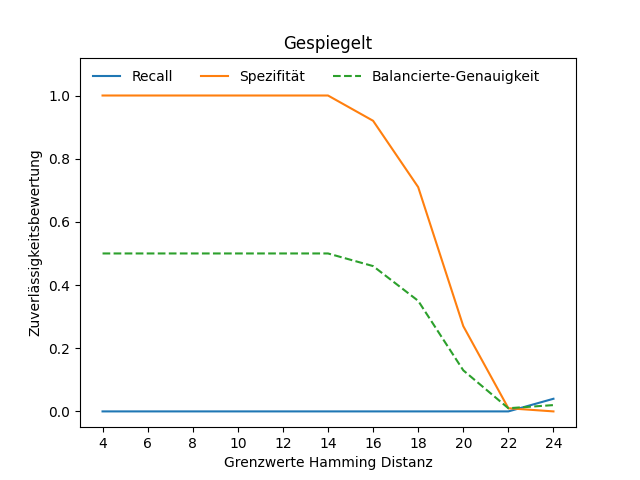
\includegraphics[scale=0.43]{Abbildungen/Evaluation/phash/mirrored}
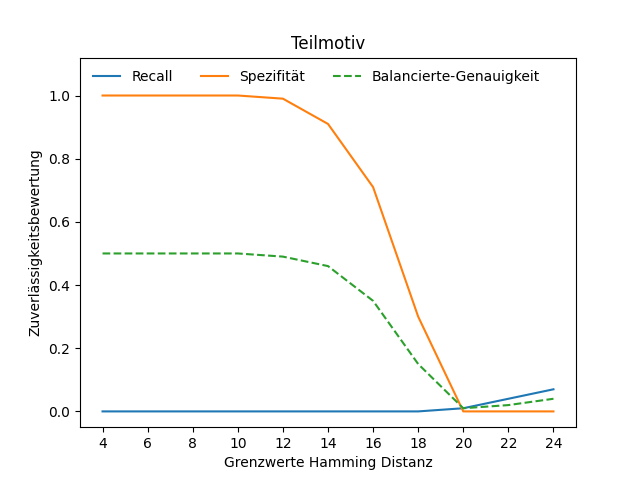
\includegraphics[scale=0.43]{Abbildungen/Evaluation/phash/part}
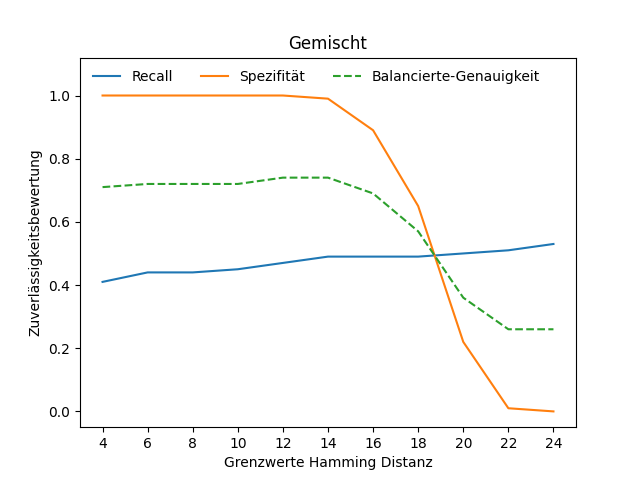
\includegraphics[scale=0.43]{Abbildungen/Evaluation/phash/mixed}
\caption{Zuverl�ssigkeit des pHash Algorithmus in mehreren Szenarien �ber mehrere Grenzwerte f�r die Hamming-Distanz}
\label{fig:phash-thresholds}
\end{figure}

In Abbildung \ref{fig:phash-standard} ist die Performance des pHash Algorithmus, der in der Spread Group eingesetzt wird, in den verschiedenen Szenarien zu sehen. 
F�r diese Tests wurde der Grenzwert f�r die Hamming-Distanz auf 4 festgelegt. 
Dieser Grenzwert wird auch in der Spread Group verwendet.

Bemerkenswert ist, dass die Spezifizit�t in allen Szenarien bei 100\% liegt. pHash ist sehr gut darin falsch-positiv Bewertungen zu vermeiden. 
Ein Unikat im Suchsatz wurde in Tests also niemals f�lschlicherweise als Duplikat erkannt. 

Was den Recall angeht, performt pHash besonders gut bei identischen, skalierten und verschobenen Kopien. 
In diesen F�llen werden die meisten Duplikate richtig erkannt. 
In allen anderen Szenarien hat pHash gro�e Schwierigkeiten Duplikate zu erkennen. 

Die hohe Zuverl�ssigkeit beim erkennen von verschoben Duplikaten, l�sst sich darauf zur�ckf�hren, dass fast alle Bilder im Suchsatz f�r dieses Szenario einen transparenten Hintergrund haben. 
Bilder mit transparenten werden von pHash auf die Gr��e ihres Motivs zugeschnitten. 
Dadurch geht die Verschiebung verloren und Duplikate k�nnen einfach erkannt werden.
Einzelne Testbilder mit opaken Hintergrund haben ergeben, dass pHash Schwierigkeiten hat Duplikate mit gro�en Verschiebungen zu erkennen. 

Der pHash Algorithmus wurde au�erdem f�r h�here Grenzwerte bei der Hamming-Distanz getestet (siehe Abbildung \ref{fig:phash-thresholds}). 
Grenzwerte bis zu 8 erh�hen den Recall mit geringen einbu�en bei der Spezifizit�t. F�r Grenzwerte bis 16 steigt der Recall noch weiter, allerdings mit h�herer Belastung der Spezifizit�t. 
Besonders die Szenarien mit Duplikaten mit ge�nderte Rotation der Motvie und ge�nderter Hintergrundfarbe profiteren von dem erh�hten Grenzwert.

Bei Grenzwerten gr��er als 16 nimmt die Reduktion der Spezifizit�t stark zu. 



